\documentclass{article}

\usepackage{fancyhdr}
\usepackage{extramarks}
\usepackage{amsmath}
\usepackage{amsthm}
\usepackage{amsfonts}
\usepackage{tikz}
\usepackage{physics}
\usepackage{amssymb}
\usepackage[plain]{algorithm}
\usepackage{algpseudocode}

\usetikzlibrary{automata,positioning}

% Basic Document Settings
%

\topmargin=-0.45in
\evensidemargin=0in
\oddsidemargin=0in
\textwidth=6.5in
\textheight=9.0in
\headsep=0.25in

\linespread{1.1}

\pagestyle{fancy}
\lhead{\hmwkAuthorName}
\chead{\hmwkClass\ : \hmwkTitle}
\rhead{\firstxmark}
\lfoot{\lastxmark}
\cfoot{\thepage}

\renewcommand\headrulewidth{0.4pt}
\renewcommand\footrulewidth{0.4pt}

\setlength\parindent{0pt}

%
% Create Problem Sections
%
\newcommand{\be}{\begin{equation}}
\newcommand{\ee}{\end{equation}}
\newcommand{\bes}{\begin{equation*}}
\newcommand{\ees}{\end{equation*}}
\newcommand{\bea}{\begin{flalign*}}
\newcommand{\eea}{\end{flalign*}}

\newcommand{\enterProblemHeader}[1]{
    \nobreak\extramarks{}{Problem \arabic{#1} continued on next page\ldots}\nobreak{}
    \nobreak\extramarks{Problem \arabic{#1} (continued)}{Problem \arabic{#1} continued on next page\ldots}\nobreak{}
}

\newcommand{\exitProblemHeader}[1]{
    \nobreak\extramarks{Problem \arabic{#1} (continued)}{Problem \arabic{#1} continued on next page\ldots}\nobreak{}
    \stepcounter{#1}
    \nobreak\extramarks{Problem \arabic{#1}}{}\nobreak{}
}

\setcounter{secnumdepth}{0}
\newcounter{partCounter}
\newcounter{homeworkProblemCounter}
\setcounter{homeworkProblemCounter}{1}
\nobreak\extramarks{Problem \arabic{homeworkProblemCounter}}{}\nobreak{}

%
% Homework Problem Environment
%
% This environment takes an optional argument. When given, it will adjust the
% problem counter. This is useful for when the problems given for your
% assignment aren't sequential. See the last 3 problems of this template for an
% example.
%
\newenvironment{homeworkProblem}[1][-1]{
    \ifnum#1>0
        \setcounter{homeworkProblemCounter}{#1}
    \fi
    \section{Problem \arabic{homeworkProblemCounter}}
    \setcounter{partCounter}{1}
    \enterProblemHeader{homeworkProblemCounter}
}{
    \exitProblemHeader{homeworkProblemCounter}
}

%
% Homework Details
%   - Title
%   - Due date
%   - Class
%   - Section/Time
%   - Instructor
%   - Author
%

\newcommand{\hmwkTitle}{Assignment\ \#5}
\newcommand{\hmwkDueDate}{Due 6th November 2018}
\newcommand{\hmwkClass}{Classical Mechanics}
\newcommand{\hmwkClassTime}{}
\newcommand{\hmwkClassInstructor}{Prof.Manas Kulkarni}
\newcommand{\hmwkAuthorName}{\textbf{Aditya Vijaykumar}}

%
% Title Page
%

\title{
    %\vspace{2in}
    \textmd{\textbf{\hmwkClass:\ \hmwkTitle}}\\
    \normalsize\vspace{0.1in}\small{\hmwkDueDate\ }\\
%    \vspace{3in}
}

\author{\hmwkAuthorName}
\date{}

\renewcommand{\part}[1]{\textbf{\large Part \Alph{partCounter}}\stepcounter{partCounter}\\}

%
% Various Helper Commands
%

% Useful for algorithms
\newcommand{\alg}[1]{\textsc{\bfseries \footnotesize #1}}

% For derivatives
\newcommand{\deriv}[1]{\frac{\mathrm{d}}{\mathrm{d}x} (#1)}

% For partial derivatives
\newcommand{\pderiv}[2]{\frac{\partial}{\partial #1} (#2)}

% Integral dx
\newcommand{\dx}{\mathrm{d}x}

% Alias for the Solution section header
\newcommand{\solution}{\textbf{\large Solution}}

% Probability commands: Expectation, Variance, Covariance, Bias
\newcommand{\E}{\mathrm{E}}
\newcommand{\Var}{\mathrm{Var}}
\newcommand{\Cov}{\mathrm{Cov}}
\newcommand{\Bias}{\mathrm{Bias}}

\begin{document}
\maketitle
The Euler Equations of motion for rotation about principal axes with moments of inertia $ I_1, I_2, I_3 $ and torques $ N_1, N_2, N_3 $ are given by,
\begin{align}
I_1 \dot{\omega}_1 - \omega_2 \omega_3 (I_2 - I_3) = N_1\\
I_2 \dot{\omega}_2 - \omega_3 \omega_1 (I_3 - I_1) = N_2\\
I_3 \dot{\omega}_3 - \omega_1 \omega_2 (I_1 - I_2) = N_3 \label{eueq}
\end{align}

\begin{homeworkProblem}[1]
	\textbf{Part (a)}\\
	\begin{figure}[h!]
		\centering
		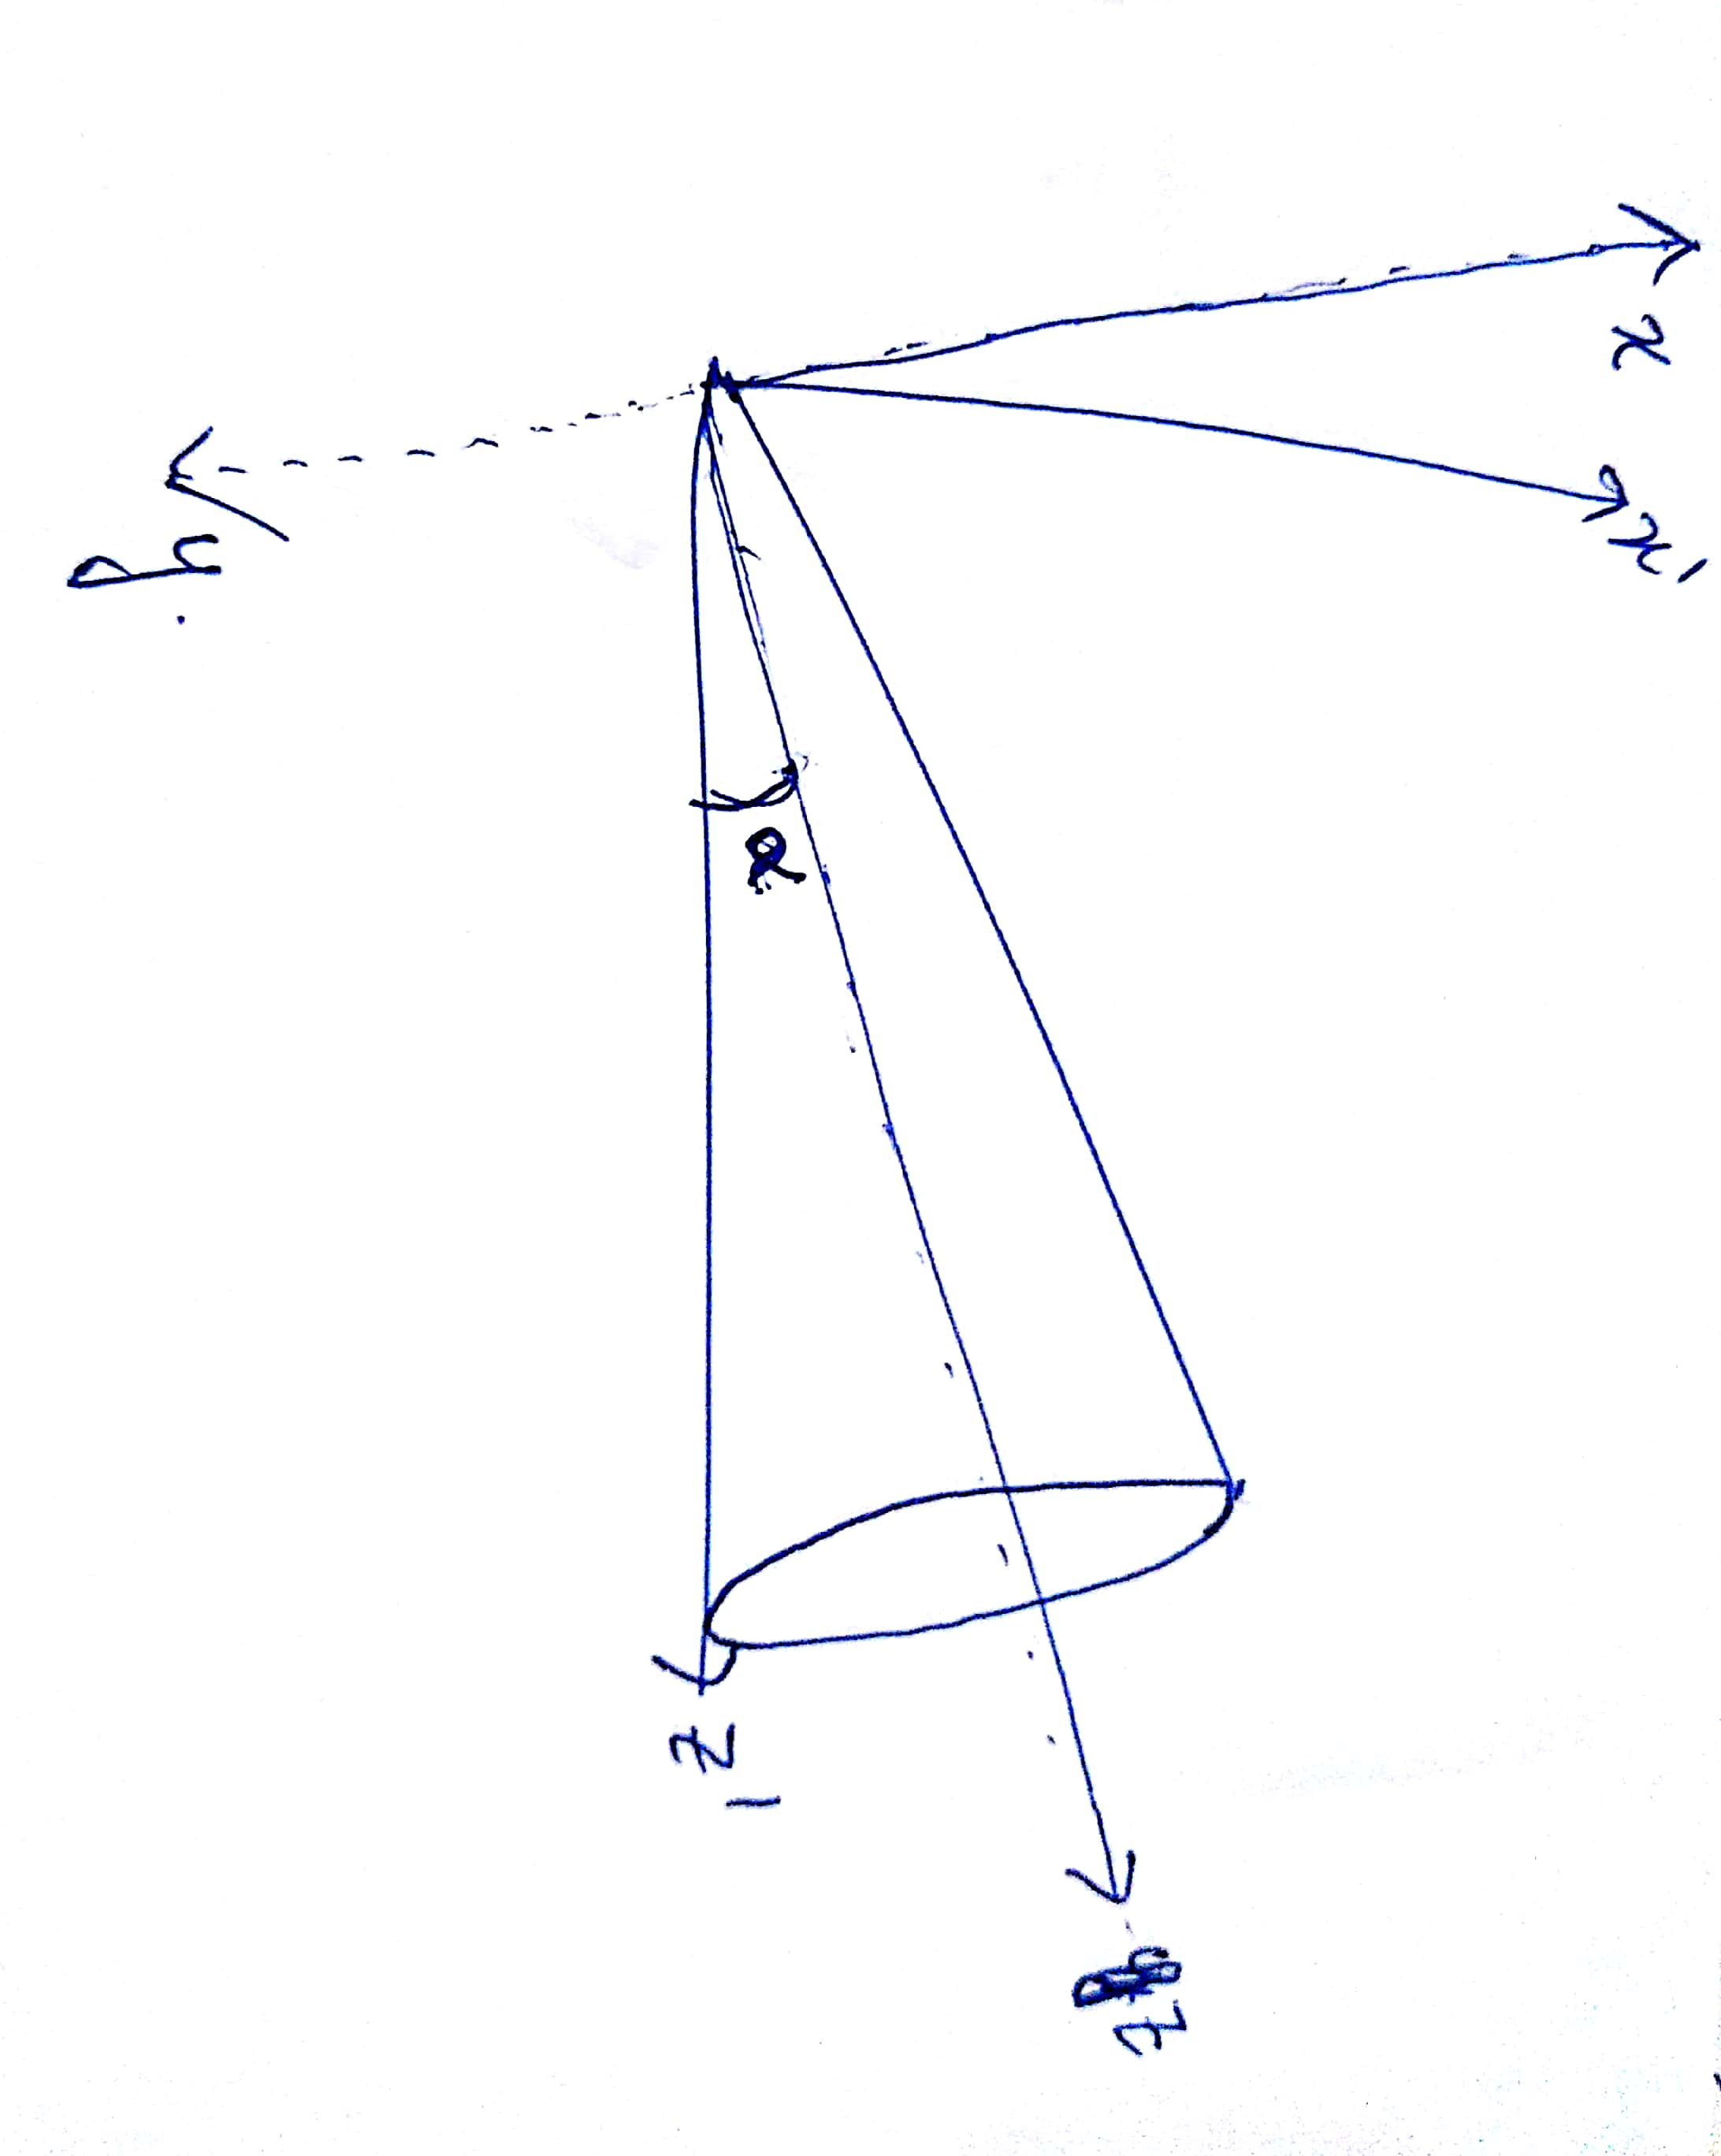
\includegraphics[scale=0.1,angle=90]{q1a.jpg}
	\end{figure}
	The moment of inertia tensor in the $ xyz $ coordinate system is given by,
	\begin{equation*}
	I =\dfrac{3mh^2}{5} \mqty[\dmat[0]{1 + \dfrac{\tan^2 \alpha}{4},1 + \dfrac{\tan^2 \alpha}{4},\dfrac{\tan^2 \alpha}{2}}]
	\end{equation*}
	As $ I $ is a tensor, we rotate the current $ I $ to the get the moment of inertia $ I' $ in the $ x'y'z' $ frame,
	\begin{align*}
	I' &= R(\alpha) I R^T(\alpha)\\
	I' &=\dfrac{3mh^2}{5} \left[
	\begin{array}{ccc}
	\left(\dfrac{\tan ^2\alpha}{4}+1\right) \cos ^2\alpha+\dfrac{1}{2} \sin ^2\alpha \tan ^2\alpha & 0 & \dfrac{1}{2} \sin ^2\alpha \tan \alpha-\cos \alpha \sin \alpha \left(\dfrac{\tan ^2\alpha}{4}+1\right) \\
	0 & \dfrac{\tan ^2\alpha}{4}+1 & 0 \\
	\dfrac{1}{2} \sin ^2\alpha \tan \alpha-\cos \alpha \sin \alpha \left(\dfrac{\tan ^2\alpha}{4}+1\right) & 0 & \left(\dfrac{\tan ^2\alpha}{4}+1\right) \sin ^2\alpha+\dfrac{\sin ^2\alpha}{2} \\
	\end{array}
	\right]
	\end{align*}
	
	The angular velocity is along the instantaneous axis of rotation, which in this case is the new $ z $ axis. The cone traces out a circle of its slant height $l = \dfrac{h}{\cos \alpha} $. Hence the angular velocity is just, 
	\begin{equation*}
	\Omega = \dfrac{2 \pi l}{\tau h \tan \alpha} = \dfrac{2\pi}{\tau \sin \alpha}
	\end{equation*}
	Hence, the angular velocity vector $ \va{\Omega} = \mqty[0 & 0 & \Omega] $. The angular momentum $ \va{L} $ is given by,
	\begin{equation*}
	\va{L} = I' \va{\Omega} = \left[
	\begin{array}{c}
	-\frac{h^3 \pi  \rho  (5 \cos (2 \alpha )+3) \tan ^2(\alpha )}{20 \tau } \\
	0 \\
	\frac{h^3 \pi  \rho  (5 \cos (2 \alpha )+7) \tan ^3(\alpha )}{20 \tau } \\
	\end{array}
	\right]
	\end{equation*}
	and the Kinetic energy $ K$ is,
	\begin{equation*}
	K = \va{\Omega}^T \va{L} = \frac{\pi ^2 h^3 \rho  (5 \cos (2 \alpha )+7) \tan ^2(\alpha )}{10 \tau ^2}
	\end{equation*}
	In both the above expressions, we have used,
	\begin{equation*}
	m = \rho \dfrac{\pi r^2 h}{3} = \rho \dfrac{\pi h^3 \tan^2 \alpha}{3} 
	\end{equation*}
	\textbf{Part (b)}\\
	The coordinates of the centre of mass of the rod are given by,
	\begin{equation*}
	x = l \sin \theta \qq{and} y = \alpha + l \cos \theta \implies \dot{x}^2 + \dot{y}^2 = \dot{\alpha}^2 + l^2 \dot{\theta}^2 - 2 l \dot{\alpha} \dot{\theta} \sin \theta
	\end{equation*}
	Let's write down the expressions for Kinetic Energy $ T $ and Potential Energy $ V $,
	\begin{align*}
	T &= \dfrac{M v_{CM}^2}{2} + \dfrac{I_{CM}\dot{\theta}^2}{2}\\
	&= \dfrac{M(\dot{x}^2 + \dot{y}^2)}{2} + \dfrac{Ml^2 \dot{\theta}^2}{6}\\
	T &= \dfrac{M(\dot{\alpha}^2 + l^2 \dot{\theta}^2 - 2 l \dot{\alpha} \dot{\theta} \sin \theta)}{2} + \dfrac{Ml^2 \dot{\theta}^2}{6}\\
	V & = - Mgy_{CM} + \dfrac{k \alpha^2}{2}\\
	&= -Mg ( \alpha + l \cos \theta ) + \dfrac{k \alpha^2}{2}
	\end{align*}
	We now write down the Lagrangian,
	\begin{equation*}
	L = \dfrac{M(\dot{\alpha}^2 + l^2 \dot{\theta}^2 - 2 l \dot{\alpha} \dot{\theta} \sin \theta)}{2} + \dfrac{Ml^2 \dot{\theta}^2}{6} + Mg ( \alpha + l \cos \theta ) - \dfrac{k \alpha^2}{2}
	\end{equation*}
	The equations of motion are,
	\begin{align*}
	\dv{t}\qty(M\dot{\alpha} - l \dot{\theta} \sin \theta)= Mg - k \alpha &\implies \ddot{\alpha} -\dfrac{l \ddot{\theta}\sin \theta  + l \dot{\theta}^2 \cos \theta}{M} - g + \dfrac{k \alpha}{M} =0 \qq{and} \\
	\dv{t}\qty(Ml^2 \dot{\theta} - l \dot{\alpha} \sin \theta + \dfrac{Ml^2 \dot{\theta} }{3}) = - Mgl \sin \theta &\implies  \dfrac{4l \ddot{\theta} }{3} - \dfrac{ \ddot{\alpha} \sin \theta + \dot{\alpha}\dot{\theta} \cos \theta}{M} + g\sin \theta = 0
	\end{align*}
\end{homeworkProblem}	













\begin{homeworkProblem}[2]
	Let $ f(q_i,t) $ be a function such that $ L'(q_i,\dot{q}_i,t) = L(q_i,\dot{q}_i,t) + \dv{f}{t} $. We have seen that the equations of motion remain unchanged by this addition.
	
	Let's first calculate the canonical momenta $ p'_i $,
	\begin{equation*}
	p'_i = \pdv{L'}{\dot{q}_i} = \pdv{L}{\dot{q}_i} + \pdv{\dot{q}_i}\qty(\dv{f}{t}) 	=   p_i + \pdv{\dot{q}_i}\qty(\dv{f}{t}) =  p_i + \pdv{\dot{q}_i}\qty(\sum_{j} \pdv{f}{{q_j}} \dot{q_j}) =  p_i +  \pdv{f}{{q_i}}
	\end{equation*}
	Let's calculate the Hamiltonian $ H'(q_i,p_i,t)  $,
	\begin{align*}
	H'(q_i,p_i,t) &= \sum_{i}\qty(p_i + \pdv{f}{{q_i}}) \dot{q}_i - L'\\
	&=  \sum_{i} p_i \dot{q}_i - L + \sum_{i} \dot{q}_i \pdv{f}{{q_i}} - \dv{f}{t}\\
	&= H(q_i,p_i,t)  +  \sum_{i} \dot{q}_i \pdv{f}{{q_i}} -\sum_{i} \dot{q}_i \pdv{f}{{q_i}}\\
	H'(q_i,p_i,t)&= H(q_i,p_i,t)
	\end{align*}
	
 	As the Hamiltonians are essentially the same, the equations of motion are same as well.\\
 	
	
	\textbf{Part (b)}\\
	Given that,
	\begin{align*}
	L &= -mc^2 \sqrt{1 - \dfrac{{v}^2}{c^2}} - e \phi + \dfrac{e}{c} \va{v}\vdot \va{A}\\
	&= -mc^2 \sqrt{1 - \dfrac{\dot{x}^2 + \dot{y}^2 + \dot{z}^2}{c^2}} - e \phi + \dfrac{e}{c} (\dot{x} A_x + \dot{y} A_y + \dot{z} A_z)\\
	&= -\dfrac{m(c^2 - \dot{x}^2 + \dot{y}^2 + \dot{z}^2)}{\sqrt{1 - \dfrac{v^2}{c^2}}} - e \phi + \dfrac{e}{c} (\dot{x} A_x + \dot{y} A_y + \dot{z} A_z)
	\end{align*}
	We first write the canonical momenta,
	\begin{equation*}
	p_x = \pdv{L}{\dot{x}} = -mc^2 \dfrac{\qty(\dfrac{-2\dot{x}}{c^2})}{2\sqrt{1 - \dfrac{{v}^2}{c^2}}} + \dfrac{e}{c}A_x = \dfrac{{m\dot{x}}}{\sqrt{1 - \dfrac{{v}^2}{c^2}}} + \dfrac{e}{c}A_x
	\end{equation*}
	Similarly,
	\begin{equation*}
	p_y = \dfrac{{m\dot{y}}}{\sqrt{1 - \dfrac{{v}^2}{c^2}}} + \dfrac{e}{c}A_y \qq{and} p_z = \dfrac{{m\dot{z}}}{\sqrt{1 - \dfrac{{v}^2}{c^2}}} + \dfrac{e}{c}A_z
	\end{equation*}
	Let's first evaluate $ \gamma = \dfrac{1}{\sqrt{1-\dfrac{v^2}{c^2}}}$.
	
	\begin{align*}
	\gamma = \dfrac{1}{\sqrt{1-\dfrac{v^2}{c^2}}} =  \dfrac{1}{\sqrt{1-\dfrac{\sum_{i = x,y,z}\dot{x}_i^2}{c^2}}}
	\end{align*}
	From the formulae of the canonical momenta, one can see that,
	\begin{align*}
	H &= p_x \dot{x} + p_y \dot{y} + p_z \dot{z} - L\\
	&= \frac{p_x \left(p_x-\frac{e A_x}{c}\right)}{\gamma  m}+\frac{p_y \left(p_y-\frac{e A_y}{c}\right)}{\gamma  m}+\frac{p_z \left(p_z-\frac{e A_z}{c}\right)}{\gamma  m} - \frac{e \left(\frac{A_x \left(p_x-\frac{e A_x}{c}\right)}{\gamma  m}+\frac{A_y \left(p_y-\frac{e A_y}{c}\right)}{\gamma  m}+\frac{A_z \left(p_z-\frac{e A_z}{c}\right)}{\gamma  m}\right)}{c} + e \phi + mc^2 \gamma\\
	&=\frac{-2 c e A_x p_x-2 c e A_y p_y-2 c e A_z p_z+e^2( A_x^2+ A_y^2+ A_z^2)  +c^2 (p_x^2+  p_y^2 + p_z^2)}{c^2 \gamma  m} +  e  \phi + mc^2 \gamma \\
	H&= \frac{c^2 \sum_{i = x,y,z} (p_i - \dfrac{e}{c}A_i)^2}{c^2 \gamma  m} +  e  \phi + mc^2 \gamma\\
	H&= \sqrt{p^2 c^2 + m^2 c^4} + e \phi
	\end{align*}
	where $ p^2 = \sum_{i = x,y,z} (p_i - \dfrac{e}{c}A_i)^2 $. This is $ \ne T+V $.
	The Hamilton equations of motion can then be written as,
	\begin{equation*}
	\dot{x}_i = \dfrac{p_i - \dfrac{e}{c}A_i}{\sqrt{p^2 c^2 + m^2 c^4} } \qq{and} \dot{p}_i= \dfrac{e}{c} \dfrac{\qty(p_i - \dfrac{e}{c}A_i) \pdv{A_i}{x_i}}{\sqrt{p^2 c^2 + m^2 c^4} } - e \pdv{\phi}{x_i}
	\end{equation*}
	
\end{homeworkProblem}









\begin{homeworkProblem}[3]
	From the torque-free Euler equations of motion, one has,
	\begin{align*}
	I_1 \dot{\omega}_1 - \omega_2 \omega_3 (I_2 - I_3) = 0\\
	I_2 \dot{\omega}_2 - \omega_3 \omega_1 (I_3 - I_1) = 0\\
	I_3 \dot{\omega}_3 - \omega_1 \omega_2 (I_1 - I_2) = 0 
	\end{align*}
	Let's say that the body is undergoing steady motion. This means,
	\begin{equation*}
	 \omega_2 \omega_3 (I_2 - I_3) = \omega_3 \omega_1 (I_3 - I_1)  = \omega_1 \omega_2 (I_1 - I_2) = 0
	\end{equation*}
	If $ I_1, I_2, I_3 $ are all different, the above condition can be satisfied if and only if two of the $ \omega $'s are zero. Hence, if the body is indeed undergoing uniform motion, it can do so only along one of the principal axes. (In general, one cannot reduce an overall non-uniform motion to uniform motion along one axis).
	
	Let $ \omega_1 $ be the non-zero angular velocity. We apply a perturbation, such that $ \omega'_1 = \omega_1 + \epsilon \Omega_1,  \omega'_2 =  \epsilon \Omega_2,  \omega'_3= \epsilon \Omega_3$. Substituting this in the Euler equations (upto first order in $ \epsilon $),
	\begin{align*}
	I_1 \dot{\Omega}_1 &= 0\\
	I_2 \dot{\Omega}_2 &= \omega_1 \Omega_3(I_3 - I_1)\\
	I_3 \dot{\Omega}_3 &= \omega_1 \Omega_2(I_1 - I_2)
	\end{align*}
	The last two equations can be differentiated with respect to $ t $ and can be written as follows,
	\begin{align*}
	\ddot{\Omega}_2 &= - \dfrac{\omega_1^2}{I_2I_3} (I_1 - I_2)(I_1 - I_3) \Omega_2 \\
	\ddot{\Omega}_3 &=  - \dfrac{\omega_1^2}{I_2I_3} (I_1 - I_3) (I_1 - I_2) \Omega_3
	\end{align*}
	We see that the $ \Omega_1 $ and $ \Omega_2 $ will oscillate with the same frequency $ \alpha = \sqrt{\dfrac{\omega_1^2}{I_2I_3} (I_1 - I_2)(I_1 - I_3)} $. The motion will be stable only when $ \alpha > 0 \implies I_1 > I_2 \qq{and} I_1 > I_3 $ or $ I_1 < I_2 \qq{and} I_1 < I_3 $.
\end{homeworkProblem}









\begin{homeworkProblem}[4]
	The sides are given to be $ 2a,2b,2c $ along $ x,y,z $. Let's first calculate the moments of inertia,
	\begin{align*}
	I_{zz} &= \rho \int_{-a}^{a} \int_{-a}^{a} \int_{-b}^{b} dx dy dz (x^2 + y^2)\\
	&= \rho(2b) \int_{-a}^{a} dx \eval{\qty(x^2 y + \dfrac{y^2}{3})}_{-a}^{a}\\
	&= \rho(2b) \eval{\qty(\dfrac{x^3}{3} (2a) + x \dfrac{2a}{3} )}_{-a}^{a}\\
	&= \dfrac{M}{8a^2b}(2b)\dfrac{8a^4}{3}\\
	I_{zz} &= \dfrac{2Ma^2}{3}
	\end{align*}
	Similarly, $ I_{yy} = I_{xx} = \dfrac{M(a^2 + b^2)}{3} $. Let's now calculate $ I_{xy} $,
	\begin{align*}
	I_{xy} &= -\rho \int_{-a}^{a} \int_{-a}^{a} \int_{-b}^{b} dx dy dz \ xy\\
	I_{xy} &=0
	\end{align*}
	Similarly, $ I_{yz} = I_{zx} = 0$. Hence $ I_{jj} $'s are the moment of inertia about principal axes. The system has no forces acting on it. We can then write down the Euler equations as follows, with $ I_{xx} = I_1, I_{yy} = I_2, I_{zz} = I_3 $
	\begin{align*}
	\dot{\omega}_1 - \omega_2 \omega_3 \qty(1 - \dfrac{2a^2}{a^2 + b^2}) &= 0\\
	\dot{\omega}_2 - \omega_3 \omega_1 \qty(\dfrac{2a^2}{a^2 + b^2} - 1) &=0\\
	\dot{\omega}_3&= 0 \implies \omega_3 = constant
	\end{align*}
	Taking the time derivative of the first equation and substituting for $ \dot{\omega}_2 $ from the second equation, we get,
	\begin{equation*}
	\ddot{\omega}_1 = - \qty[\omega_3\qty(1 - \dfrac{2a^2}{a^2 + b^2})]^2 \omega_1 \implies \qq{periodic motion with frequency}\omega= \omega_3 \abs{1 - \dfrac{2a^2}{a^2 + b^2}}
	\end{equation*}
	As the problem is symmetric about the $ x $ and $ y $ axes, the motion will be periodic about the $ y $ axis too.
\end{homeworkProblem}
\end{document}
